\documentclass[aspectratio=169,11pt]{beamer}

% ── Packages ────────────────────────────────────────────────────────────────
\usepackage[T1]{fontenc}
\usepackage[utf8]{inputenc}
\usepackage{lmodern}
\usepackage{microtype}
\usepackage{graphicx}
\usepackage{booktabs}
\usepackage{colortbl}
\usepackage{xcolor}
\usepackage{tikz}
\usepackage{pgfplots}
\usepackage{amsmath,amssymb}
\usepackage{fontawesome5}
\usepackage{tcolorbox}
\usepackage{multicol}
\usepackage{array}
\usepackage{tabularx}
\usepackage{adjustbox}
\usepackage{setspace}
\usepackage{hyperref}

\usetikzlibrary{arrows.meta,shapes.geometric,positioning,fit,
                decorations.pathreplacing,calc,backgrounds,shadows.blur}
\pgfplotsset{compat=1.18}

\tcbuselibrary{skins,breakable}

% ── Colour palette ──────────────────────────────────────────────────────────
\definecolor{NavyPrimary}{RGB}{15,76,129}
\definecolor{NavyLight}{RGB}{26,106,181}
\definecolor{NavyDark}{RGB}{10,58,102}
\definecolor{AmberAccent}{RGB}{244,162,97}
\definecolor{AmberDark}{RGB}{220,130,60}
\definecolor{CreamBg}{RGB}{250,250,247}
\definecolor{GrayMid}{RGB}{107,114,128}
\definecolor{GrayLight}{RGB}{229,231,235}
\definecolor{SuccessGreen}{RGB}{34,197,94}
\definecolor{DangerRed}{RGB}{239,68,68}
\definecolor{InfoBlue}{RGB}{59,130,246}

% ── Beamer theme ────────────────────────────────────────────────────────────
\usetheme{default}
\usecolortheme{default}
\setbeamertemplate{navigation symbols}{}
\setbeamertemplate{itemize items}{\color{AmberAccent}\faChevronRight}
\setbeamertemplate{itemize subitem}{\color{NavyLight}\faMinus}

\setbeamercolor{background canvas}{bg=CreamBg}
\setbeamercolor{normal text}{fg=NavyDark}
\setbeamercolor{frametitle}{fg=white,bg=NavyPrimary}
\setbeamercolor{framesubtitle}{fg=AmberAccent}
\setbeamercolor{title}{fg=white}
\setbeamercolor{subtitle}{fg=AmberAccent}
\setbeamercolor{author}{fg=white}
\setbeamercolor{institute}{fg=AmberAccent}
\setbeamercolor{date}{fg=GrayLight}
\setbeamercolor{item}{fg=AmberAccent}
\setbeamercolor{block title}{bg=NavyPrimary,fg=white}
\setbeamercolor{block body}{bg=NavyPrimary!8,fg=NavyDark}
\setbeamercolor{alerted text}{fg=AmberDark}

% Tighter typography — fits content within 9.0cm available content height
\setbeamerfont{frametitle}{size=\large,series=\bfseries}
\setbeamerfont{title}{size=\LARGE,series=\bfseries}
\setbeamerfont{subtitle}{size=\normalsize}
\setbeamerfont{itemize/enumerate body}{size=\footnotesize}
\setbeamerfont{itemize/enumerate subbody}{size=\scriptsize}

% Tighter list defaults — applied at \begin{itemize}
\AtBeginEnvironment{itemize}{\setlength{\itemsep}{2pt}\setlength{\parskip}{0pt}}
\AtBeginEnvironment{enumerate}{\setlength{\itemsep}{2pt}\setlength{\parskip}{0pt}}

% Smaller margins on the frame title bar so we get more body height
\setbeamertemplate{frametitle}{%
  \nointerlineskip%
  \begin{beamercolorbox}[wd=\paperwidth,ht=2.6ex,dp=1.0ex,leftskip=0.6em,rightskip=0.6em]{frametitle}%
    \usebeamerfont{frametitle}\insertframetitle%
  \end{beamercolorbox}%
}

% ── Footer (minimal) ────────────────────────────────────────────────────────
\setbeamertemplate{footline}{%
  \hfill\color{GrayMid}\scriptsize
  \insertframenumber\,/\,\inserttotalframenumber%
  \hspace*{6pt}\vspace*{4pt}%
}

% ── tcolorbox styles ────────────────────────────────────────────────────────
% Titled boxes use an inline title band (top of the box) instead of the
% floated `attach boxed title to top left` style, which silently clipped at
% tight top-padding values and dropped titles in the rendered PDF.
\tcbset{
  navybox/.style={
    enhanced, colback=NavyPrimary!8, colframe=NavyPrimary,
    boxrule=0.6pt, arc=3pt, left=5pt, right=5pt, top=3pt, bottom=3pt,
    fonttitle=\footnotesize\bfseries, coltitle=white,
    colbacktitle=NavyPrimary,
    toptitle=1pt, bottomtitle=1pt,
    titlerule=0pt
  },
  amberbox/.style={
    enhanced, colback=AmberAccent!15, colframe=AmberDark,
    boxrule=0.6pt, arc=3pt, left=5pt, right=5pt, top=3pt, bottom=3pt
  },
  greenbox/.style={
    enhanced, colback=SuccessGreen!10, colframe=SuccessGreen!65,
    boxrule=0.6pt, arc=3pt, left=5pt, right=5pt, top=3pt, bottom=3pt,
    fonttitle=\footnotesize\bfseries, coltitle=white,
    colbacktitle=SuccessGreen!65,
    toptitle=1pt, bottomtitle=1pt, titlerule=0pt
  },
  redbox/.style={
    enhanced, colback=DangerRed!8, colframe=DangerRed!55,
    boxrule=0.6pt, arc=3pt, left=5pt, right=5pt, top=3pt, bottom=3pt,
    fonttitle=\footnotesize\bfseries, coltitle=white,
    colbacktitle=DangerRed!55,
    toptitle=1pt, bottomtitle=1pt, titlerule=0pt
  },
  statbox/.style={
    enhanced, colback=NavyPrimary, colframe=NavyDark,
    boxrule=0pt, arc=4pt, left=4pt, right=4pt, top=4pt, bottom=4pt,
    halign=center, fontupper=\color{white}
  },
  graybox/.style={
    enhanced, colback=GrayLight!40, colframe=GrayMid,
    boxrule=0.5pt, arc=3pt, left=4pt, right=4pt, top=3pt, bottom=3pt
  }
}

% ── Helpers ─────────────────────────────────────────────────────────────────
\newcommand{\highlight}[1]{\textcolor{AmberDark}{\textbf{#1}}}
\newcommand{\navy}[1]{\textcolor{NavyPrimary}{\textbf{#1}}}
\newcommand{\greentext}[1]{\textcolor{SuccessGreen!80!black}{\textbf{#1}}}
\newcommand{\redtext}[1]{\textcolor{DangerRed}{\textbf{#1}}}
\newcommand{\fig}[2][0.95\linewidth]{%
  \includegraphics[width=#1,keepaspectratio]{../results/figures/#2}}
\newcommand{\rupee}{\faRupeeSign\,}
% Force a ~tight gap below the (smaller) frametitle bar
\newcommand{\toptight}{\vspace{-0.15cm}}

% ── Title metadata ──────────────────────────────────────────────────────────
\title{Causal Impact of Bihar's 2016 Alcohol Prohibition}
\subtitle{A Synthetic Control \& Bayesian Structural Time Series Analysis}
\author{Mohammed Talha Ansari \\ \small Roll No.\ 23322016}
\institute{BS-MS Economics \\ Indian Institute of Technology Roorkee}
\date{HST-102: Time Series Analysis \quad|\quad May 2026}

% ════════════════════════════════════════════════════════════════════════════
\begin{document}
% ════════════════════════════════════════════════════════════════════════════

% ── SLIDE 1: Title ──────────────────────────────────────────────────────────
{
\setbeamertemplate{footline}{}
\setbeamercolor{background canvas}{bg=NavyPrimary}
\begin{frame}[plain]
  \begin{tikzpicture}[remember picture,overlay]
    \fill[NavyLight,opacity=0.18]
      ([xshift=-2cm,yshift=2cm]current page.south east) circle (5.5cm);
    \fill[NavyDark,opacity=0.55]
      (current page.north west) --
      ([xshift=4.5cm]current page.north west) ..
      controls ([xshift=2.5cm,yshift=-3cm]current page.north west)
           and ([xshift=2.5cm,yshift=3cm]current page.south west) ..
      ([xshift=3.5cm]current page.south west) --
      (current page.south west) -- cycle;
    \draw[AmberAccent,line width=2pt]
      ([xshift=0.85cm,yshift=-1.4cm]current page.north west) --
      ([xshift=0.85cm,yshift=1.4cm]current page.south west);
    \draw[AmberAccent,opacity=0.6,line width=0.4pt]
      ([xshift=0.85cm,yshift=-1.2cm]current page.north west) --
      ([xshift=-1cm,yshift=-1.2cm]current page.north east);
  \end{tikzpicture}

  \vspace{0.7cm}
  \begin{columns}[T,onlytextwidth]
    \column{0.62\textwidth}
      {\color{white}\fontsize{22}{26}\selectfont\bfseries
       Causal Impact of Bihar's\par}
      \vspace{0.10cm}
      {\color{AmberAccent}\fontsize{22}{26}\selectfont\bfseries
       2016 Alcohol Prohibition\par}
      \vspace{0.45cm}
      {\color{GrayLight}\small\itshape
       A Synthetic Control \& Bayesian Structural\\
       Time Series Analysis\par}
      \vspace{0.85cm}
      {\color{white}\small\bfseries Mohammed Talha Ansari}\hspace{0.5em}%
      {\color{AmberAccent}\small\textbar}\hspace{0.5em}%
      {\color{GrayLight}\small\texttt{23322016}}\par
      \vspace{0.12cm}
      {\color{GrayLight}\footnotesize BS-MS Economics, IIT Roorkee}\par
      \vspace{0.04cm}
      {\color{GrayLight}\footnotesize HST-102 Time Series Analysis}\par
      \vspace{0.85cm}
      {\color{GrayLight}\scriptsize
        \faCalendar\enspace May 2026
        \hspace{1em}\textcolor{AmberAccent}{\textbar}\hspace{1em}
        \faGithub\enspace\texttt{amsorrytola/scm-policy-india-}\par}

    \column{0.36\textwidth}
      \vspace{0.1cm}\centering
      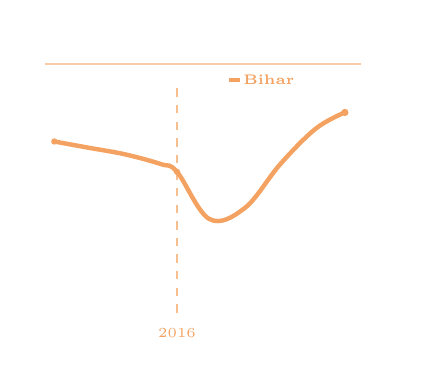
\begin{tikzpicture}[scale=0.82]
        \draw[white,opacity=0.18,line width=0.6pt,rounded corners=6pt]
          (-0.4,-0.6) rectangle (5.0,4.4);
        \node[white,opacity=0.85,font=\scriptsize\bfseries,anchor=west]
          at (-0.15,4.05) {Road accident deaths --- Bihar};
        \draw[AmberAccent,opacity=0.55,line width=0.4pt]
          (-0.15,3.85) -- (4.75,3.85);
        \draw[white,opacity=0.35,line width=0.4pt] (0,0) -- (4.6,0);
        \draw[white,opacity=0.35,line width=0.4pt] (0,0) -- (0,3.5);
        \draw[AmberAccent,dashed,opacity=0.7,line width=0.7pt]
          (1.9,0) -- (1.9,3.5);
        \node[AmberAccent,font=\tiny] at (1.9,-0.32) {2016};
        \draw[white,opacity=0.7,dashed,line width=1pt]
          plot[smooth,tension=0.7] coordinates {
            (0,2.55) (0.55,2.45) (1.1,2.32) (1.65,2.20)
            (1.9,2.18) (2.4,2.05) (2.95,1.92) (3.5,1.85)
            (4.05,1.86) (4.5,1.92)};
        \draw[AmberAccent,line width=1.6pt]
          plot[smooth,tension=0.6] coordinates {
            (0,2.65) (0.55,2.55) (1.1,2.45) (1.65,2.30)
            (1.9,2.18) (2.4,1.45) (2.95,1.62) (3.5,2.30)
            (4.05,2.85) (4.5,3.10)};
        \fill[AmberAccent] (0,2.65) circle (1.4pt);
        \fill[AmberAccent] (1.9,2.18) circle (1.4pt);
        \fill[AmberAccent] (4.5,3.10) circle (1.6pt);
        \node[AmberAccent,font=\tiny\bfseries,anchor=west]
          at (2.55,3.6) {\rule[0.5ex]{4pt}{1.4pt}\,Bihar};
        \node[white,opacity=0.7,font=\tiny,anchor=west]
          at (3.55,3.6) {\rule[0.5ex]{4pt}{0.8pt}\,Synthetic};
      \end{tikzpicture}
  \end{columns}
\end{frame}
}

% ── SLIDE 2: Outline ────────────────────────────────────────────────────────
\begin{frame}{Outline}
  \toptight
  \vspace{0.4cm}
  \begin{columns}[T,onlytextwidth]
    \column{0.48\textwidth}
      \begin{tcolorbox}[navybox,title={\faMap\enspace Part I --- Setup}]
        \footnotesize\setlength\itemsep{2pt}
        \textbf{1.} Motivation \& policy context\\[2pt]
        \textbf{2.} Research questions\\[2pt]
        \textbf{3.} Identification challenge\\[2pt]
        \textbf{4.} Data \& panel construction
      \end{tcolorbox}
      \vspace{0.30cm}
      \begin{tcolorbox}[navybox,title={\faCalculator\enspace Part II --- Methodology}]
        \footnotesize
        \textbf{5.} Synthetic Control Method\\[2pt]
        \textbf{6.} Convex hull problem \& fix\\[2pt]
        \textbf{7.} Bayesian Structural Time Series
      \end{tcolorbox}

    \column{0.48\textwidth}
      \begin{tcolorbox}[navybox,title={\faChartLine\enspace Part III --- Results}]
        \footnotesize
        \textbf{8.} Road-accident deaths (primary)\\[2pt]
        \textbf{9.} Own tax revenue (fiscal proxy)\\[2pt]
        \textbf{10.} NSDP per-capita growth\\[2pt]
        \textbf{11.} Cross-outcome synthesis
      \end{tcolorbox}
      \vspace{0.30cm}
      \begin{tcolorbox}[navybox,title={\faShield*\enspace Part IV --- Closing}]
        \footnotesize
        \textbf{12.} Robustness \& limitations\\[2pt]
        \textbf{13.} Interactive website demo\\[2pt]
        \textbf{14.} Conclusions \& Q\,\&\,A
      \end{tcolorbox}
  \end{columns}
\end{frame}

% ── SLIDE 3: Motivation ─────────────────────────────────────────────────────
\begin{frame}{Motivation --- Why Study Bihar's Prohibition?}
  \toptight
  \begin{columns}[T,onlytextwidth]
    \column{0.55\textwidth}
      \begin{tcolorbox}[amberbox]
        \footnotesize\textbf{The policy.} Effective \highlight{April 5, 2016},
        Bihar enacted total prohibition on the sale and consumption of
        alcohol --- the largest sub-national prohibition by population in
        modern history (\textasciitilde 120M people).
      \end{tcolorbox}
      \vspace{0.25cm}
      \textbf{\navy{\small Why this case is methodologically interesting:}}
      \begin{itemize}
        \item Sharp, well-dated discontinuity --- ideal for causal designs
        \item Single treated unit $\Rightarrow$ DiD parallel-trends hard to
              defend; SCM is the natural choice
        \item Multiple competing channels (safety, fiscal, economic) ---
              direction of net effect is empirical
      \end{itemize}

    \column{0.40\textwidth}
      \begin{tcolorbox}[statbox,width=\linewidth]
        \fontsize{22}{26}\selectfont\bfseries\color{AmberAccent}120M\\
        \scriptsize\color{white}affected population
      \end{tcolorbox}
      \vspace{0.18cm}
      \begin{tcolorbox}[statbox,width=\linewidth]
        \fontsize{22}{26}\selectfont\bfseries\color{AmberAccent}\rupee 4{,}000\,Cr\\
        \scriptsize\color{white}pre-prohibition state excise (FY15--16)
      \end{tcolorbox}
      \vspace{0.18cm}
      \begin{tcolorbox}[statbox,width=\linewidth]
        \fontsize{22}{26}\selectfont\bfseries\color{AmberAccent}3 outcomes\\
        \scriptsize\color{white}safety / fiscal / economic
      \end{tcolorbox}
  \end{columns}
\end{frame}

% ── SLIDE 4: Research Questions ─────────────────────────────────────────────
\begin{frame}{Research Questions}
  \toptight
  \vspace{0.2cm}
  \begin{tcolorbox}[navybox,title={\faQuestion\enspace Three questions, one identification strategy}]
    \footnotesize
    \begin{enumerate}\setlength\itemsep{4pt}
      \item Did prohibition \highlight{reduce road-accident deaths}
            relative to a counterfactual Bihar that did not enact prohibition?
      \item Did prohibition \highlight{reduce state own-tax revenue} via the
            loss of the excise component?
      \item Did prohibition \highlight{accelerate or depress per-capita
            growth} relative to comparable states?
    \end{enumerate}
  \end{tcolorbox}

  \vspace{0.35cm}
  {\small\textbf{\navy{Identification.}}\;
  Construct a \emph{synthetic Bihar} as a weighted average of donor states
  whose pre-2016 trajectory tracks Bihar's, then read the post-2016 gap as
  the treatment effect. Triangulate with a Bayesian structural counterfactual
  (BSTS).}

  \vspace{0.30cm}
  \begin{tcolorbox}[greenbox]
    \scriptsize\textbf{Why three outcomes?} Each isolates a distinct welfare
    dimension --- Q1 the \greentext{intended public-health} gain,
    Q2 the \redtext{direct fiscal cost}, Q3 the \emph{net} economic effect
    of competing channels.
  \end{tcolorbox}
\end{frame}

% ── SLIDE 5: Identification Challenge ───────────────────────────────────────
\begin{frame}{The Identification Challenge}
  \toptight
  \begin{columns}[T,onlytextwidth]
    \column{0.48\textwidth}
      \textbf{\navy{\small Standard tools fall short.}}
      \begin{itemize}
        \item \redtext{DiD} requires parallel pre-trends --- Bihar is an
              outlier on income, urbanisation, literacy
        \item \redtext{IV} has no obvious instrument for state-wide policy
        \item Single treated unit $\Rightarrow$ no within-treatment variation
      \end{itemize}
      \vspace{0.30cm}
      \begin{tcolorbox}[amberbox]
        \scriptsize\textbf{SCM matches the structure.}
        \highlight{One treated unit, many donors, long pre-period} ---
        exactly the setting Abadie--Diamond--Hainmueller (2010) introduced
        the method for.
      \end{tcolorbox}

    \column{0.48\textwidth}
      \begin{tcolorbox}[navybox,title={\faExclamationTriangle\enspace Convex hull caveat}]
        \scriptsize Bihar's pre-period income and urbanisation lie at the
        \emph{lower edge} of the donor pool. A naive SCM optimiser collapses
        to a \redtext{corner solution} (100\% UP weight).
        \vspace{0.15cm}\\
        \emph{Fix:} include lagged outcomes as
        \texttt{special\_predictors} (Abadie 2010 §IV) --- this anchors the
        synthetic to Bihar's actual trajectory, not just its socio-economic
        profile.
      \end{tcolorbox}
  \end{columns}
\end{frame}

% ── SLIDE 6: Data Sources ───────────────────────────────────────────────────
\begin{frame}{Data --- Panel Construction}
  \toptight
  {\footnotesize\textbf{\navy{Annual state panel, 2010--2022}} ---
   15 states $\times$ 13 years $=$ 195 obs.
   Telangana excluded (only 2 pre-treatment obs after 2014 bifurcation).}

  \vspace{0.25cm}
  \scriptsize
  \begin{tabularx}{\linewidth}{@{}lXl@{}}
    \toprule
    \rowcolor{NavyPrimary}\color{white}\textbf{Variable} &
    \color{white}\textbf{Description} &
    \color{white}\textbf{Source} \\
    \midrule
    \texttt{road\_accident\_deaths} & Persons killed in road accidents
      & MoRTH PDFs 2010--23\\
    \texttt{own\_tax\_revenue\_cr} & State own-tax revenue (composite, \rupee Cr)
      & RBI Handbook T168\\
    \texttt{nsdp\_pc\_current\_inr} & Net State Domestic Product per capita
      & RBI Handbook T19\\
    \texttt{nsdp\_growth\_yoy} & YoY \% growth of NSDP per capita (derived)
      & Computed from T19\\
    \texttt{urban\_share\_pct} & Urban population share
      & Census 2011 + interp.\\
    \texttt{literacy\_rate\_pct} & Literacy rate (age 7+)
      & Census 2011 + interp.\\
    \bottomrule
  \end{tabularx}

  \vspace{0.4cm}
  \begin{tcolorbox}[graybox]
    \scriptsize\textbf{Acquisition stack.} MoRTH PDFs via Wayback CDX
    $\rightarrow$ \texttt{camelot} stream-mode extraction. RBI behind F5
    BIG-IP TSPD cookie wall --- two-step warmup. Full provenance log:
    \texttt{data/raw/bihar/SOURCES.md}.
  \end{tcolorbox}
\end{frame}

% ── SLIDE 7: EDA ────────────────────────────────────────────────────────────
\begin{frame}{Pre-Treatment EDA --- Donor Selection}
  \toptight
  \begin{columns}[T,onlytextwidth]
    \column{0.58\textwidth}
      \centering
      \fig[\linewidth]{eda_bihar_pretrend_top5.png}

    \column{0.40\textwidth}
      \textbf{\navy{\small Top correlated donors (pre-2016):}}
      \begin{itemize}
        \item Jharkhand, Odisha, UP, MP, West Bengal
        \item Geographic neighbours \& similar income trajectories
        \item Pre-period $r > 0.9$ for top 3
      \end{itemize}
      \vspace{0.18cm}
      \begin{tcolorbox}[amberbox]
        \scriptsize\textbf{Why this matters.} Donor pool must span Bihar's
        pre-trend in \emph{outcome space}. Selecting on outcome correlation
        is more robust than selecting on covariates alone.
      \end{tcolorbox}
  \end{columns}
\end{frame}

% ── SLIDE 8: SCM Method ─────────────────────────────────────────────────────
\begin{frame}{Method --- Synthetic Control}
  \toptight
  {\footnotesize Treated unit $i=1$ (Bihar) and $J$ donors. Choose weights
  $\mathbf{w}=(w_2,\dots,w_{J+1})^\top$ to solve:}

  \vspace{0.05cm}
  \begin{tcolorbox}[navybox]
    \centering\small
    $\displaystyle
      \mathbf{w}^* \;=\; \arg\min_{\mathbf{w}\in\mathcal{W}}\;
      \bigl\| X_1 - X_0\,\mathbf{w} \bigr\|_V \,,\quad
      \mathcal{W}=\Bigl\{\mathbf{w}\!:\!w_j\ge 0,\;\sum w_j=1\Bigr\}$
  \end{tcolorbox}

  \vspace{0.10cm}
  \scriptsize
  $X_1$: predictor vector for treated; $X_0$: $K\times J$ donor matrix; $V$:
  predictor-importance weight matrix (chosen to minimise pre-period MSPE).

  \vspace{0.30cm}
  \textbf{\navy{\footnotesize Two consequences of the convex-hull constraint:}}
  \begin{itemize}
    \item Synthetic Bihar cannot extrapolate beyond the donor envelope ---
          good for honest counterfactuals
    \item Near a corner, weights collapse to a single donor $\Rightarrow$
          poor pre-fit + spurious post-period gap
  \end{itemize}
\end{frame}

% ── SLIDE 9: Convex Hull Problem ────────────────────────────────────────────
\begin{frame}{The Convex Hull Problem --- And Its Fix}
  \toptight
  \begin{columns}[T,onlytextwidth]
    \column{0.50\textwidth}
      \centering
      \fig[\linewidth]{eda_bihar_vs_donor_avg.png}\\[2pt]
      \scriptsize\color{GrayMid} Bihar persistently \emph{below} the donor
      pool average on road-accident deaths.

    \column{0.46\textwidth}
      \textbf{\navy{\small Without the fix.}}
      \begin{itemize}
        \item Match on socio-economic predictors only
        \item Optimiser picks 100\% UP weight
        \item Pre-RMSPE \redtext{$\sim$1{,}300 deaths}; post gap meaningless
      \end{itemize}
      \vspace{0.20cm}
      \textbf{\navy{\small With lagged-outcome anchoring (Abadie 2010 §IV).}}
      \begin{itemize}
        \item Each pre-period year's outcome $\to$ a
              \texttt{special\_predictor}
        \item Pre-RMSPE drops to \greentext{42 deaths} ($<\!1\%$ of mean)
              --- excellent fit
      \end{itemize}
  \end{columns}
\end{frame}

% ── SLIDE 10: SCM Main Result ───────────────────────────────────────────────
\begin{frame}{Result --- Bihar vs Synthetic Bihar (Road Deaths)}
  \toptight
  \centering
  \fig[0.70\linewidth]{scm_bihar_main.png}

  \vspace{0.15cm}
  \begin{columns}[T,onlytextwidth]
    \column{0.32\textwidth}
      \begin{tcolorbox}[statbox]
        \large\bfseries\color{AmberAccent}22.87$\boldsymbol{\times}$\\
        \scriptsize\color{white} RMSPE ratio (post/pre)
      \end{tcolorbox}
    \column{0.32\textwidth}
      \begin{tcolorbox}[statbox]
        \large\bfseries\color{AmberAccent}+360 / yr\\
        \scriptsize\color{white} avg post-treatment gap (deaths)
      \end{tcolorbox}
    \column{0.32\textwidth}
      \begin{tcolorbox}[statbox]
        \large\bfseries\color{AmberAccent}p $\approx$ 0.071\\
        \scriptsize\color{white} permutation, rank 2 / 14
      \end{tcolorbox}
  \end{columns}
\end{frame}

% ── SLIDE 11: Gap Plot ──────────────────────────────────────────────────────
\begin{frame}{Treatment Effect --- Year by Year}
  \toptight
  \begin{columns}[T,onlytextwidth]
    \column{0.55\textwidth}
      \centering
      \fig[\linewidth]{scm_bihar_gap.png}

    \column{0.42\textwidth}
      \textbf{\navy{\small Two distinct phases:}}\\[4pt]
      \begin{tcolorbox}[greenbox]
        \scriptsize\textbf{2016--2017 (lives saved).}
        $\sim$600--900 fewer deaths than counterfactual; consistent with
        immediate compliance.
      \end{tcolorbox}
      \vspace{0.15cm}
      \begin{tcolorbox}[redbox]
        \scriptsize\textbf{2018--2022 (effect reverses).}
        Bihar climbs above synthetic by +1{,}000 to +3{,}300 deaths/yr ---
        consistent with illicit-market substitution and weaker enforcement.
      \end{tcolorbox}
      \vspace{0.15cm}
      \begin{tcolorbox}[amberbox]
        \scriptsize \textbf{Donor weights:}
        \highlight{Jharkhand 0.68}, Odisha 0.16, UP 0.16.
      \end{tcolorbox}
  \end{columns}
\end{frame}

% ── SLIDE 12: Placebo Inference ─────────────────────────────────────────────
\begin{frame}{Inference --- In-Space Placebo}
  \toptight
  \begin{columns}[T,onlytextwidth]
    \column{0.60\textwidth}
      \centering
      \fig[\linewidth]{scm_bihar_placebo.png}

    \column{0.37\textwidth}
      \textbf{\navy{\small Permutation test.}}\\[4pt]
      {\footnotesize Refit SCM treating each of 13 donors as if treated.
      Bihar's gap (navy) should stand out from placebos (gray) if the effect
      is real.}
      \vspace{0.25cm}
      \begin{tcolorbox}[statbox]
        \large\bfseries\color{AmberAccent} Rank 2 / 14\\
        \scriptsize\color{white} p $\approx$ 0.071
      \end{tcolorbox}
      \vspace{0.18cm}
      {\scriptsize Only Maharashtra has a larger ratio --- consistent with
      its own outlier post-2018 trajectory unrelated to alcohol policy.}
  \end{columns}
\end{frame}

% ── SLIDE 13: Leave-One-Out ─────────────────────────────────────────────────
\begin{frame}{Robustness --- Leave-One-Out}
  \toptight
  \begin{columns}[T,onlytextwidth]
    \column{0.60\textwidth}
      \centering
      \fig[\linewidth]{scm_bihar_loo.png}

    \column{0.37\textwidth}
      \textbf{\navy{\small Drop each donor in turn.}}\\[4pt]
      {\footnotesize If a single donor were driving the result, removing it
      would collapse the synthetic. Instead all 13 LOO refits trace nearly
      the same trajectory.}
      \vspace{0.30cm}
      \begin{tcolorbox}[greenbox]
        \scriptsize Result is \greentext{not driven by any single donor}
        --- including dropping the dominant Jharkhand weight produces a
        materially identical synthetic.
      \end{tcolorbox}
  \end{columns}
\end{frame}

% ── SLIDE 14: BSTS Method ───────────────────────────────────────────────────
\begin{frame}{Method --- Bayesian Structural Time Series}
  \toptight
  {\footnotesize Brodersen et al.\ (2015) decompose the observed series as:}

  \vspace{0.05cm}
  \begin{tcolorbox}[navybox]
    \centering\small
    $y_t \;=\; \mu_t \;+\; \tau_t \;+\; \boldsymbol{\beta}^\top
              \mathbf{x}_t \;+\; \varepsilon_t$
  \end{tcolorbox}

  \vspace{0.05cm}
  \scriptsize $\mu_t$: local-level trend $\;|\;$
  $\tau_t$: seasonality (omitted, annual data) $\;|\;$
  $\boldsymbol{\beta}^\top\mathbf{x}_t$: regression on donor outcomes
  with \emph{spike-and-slab} priors $\;|\;$
  $\varepsilon_t \sim \mathcal{N}(0,\sigma^2)$.

  \vspace{0.30cm}
  \textbf{\navy{\footnotesize Why BSTS triangulates with SCM:}}
  \begin{itemize}
    \item Different functional form (linear regression with priors vs.\
          convex average) $\Rightarrow$ different mis-specification risks
    \item Yields full posterior $\Rightarrow$ credible intervals
    \item Caveat: with $n_\text{pre}=6 \ll J=13$ the regression overfits
          $\Rightarrow$ restrict to top-$k$ donors via correlation
          (\texttt{max\_donors=3}, Brodersen §3.2)
  \end{itemize}
\end{frame}

% ── SLIDE 15: BSTS Result ───────────────────────────────────────────────────
\begin{frame}{BSTS Result --- Road-Accident Deaths}
  \toptight
  \centering
  \fig[0.56\linewidth]{bsts_bihar_main.png}

  \vspace{0.05cm}
  \begin{columns}[T,onlytextwidth]
    \column{0.48\textwidth}
      \begin{tcolorbox}[graybox]
        \scriptsize \textbf{Donors:} Haryana ($r=0.82$), Odisha ($r=0.67$),
        West Bengal ($r=0.63$).
      \end{tcolorbox}
    \column{0.48\textwidth}
      \begin{tcolorbox}[amberbox]
        \scriptsize \textbf{Avg posterior effect:} \highlight{+1{,}076 deaths/yr}
        --- larger than SCM (+360); BSTS weights post-2020 divergence fully.
      \end{tcolorbox}
  \end{columns}
\end{frame}

% ── SLIDE 16: SCM vs BSTS ───────────────────────────────────────────────────
\begin{frame}{Triangulation --- SCM vs BSTS}
  \toptight
  \centering
  \fig[0.66\linewidth]{bihar_scm_vs_bsts.png}

  \vspace{0.15cm}
  \begin{columns}[T,onlytextwidth]
    \column{0.32\textwidth}
      \begin{tcolorbox}[statbox]
        \small\bfseries\color{AmberAccent} Sign\\
        \scriptsize\color{white} Both negative 2016--17, both positive 2018+
      \end{tcolorbox}
    \column{0.32\textwidth}
      \begin{tcolorbox}[statbox]
        \small\bfseries\color{AmberAccent} Direction\\
        \scriptsize\color{white} Agree year-by-year (10/10)
      \end{tcolorbox}
    \column{0.32\textwidth}
      \begin{tcolorbox}[statbox]
        \small\bfseries\color{AmberAccent} Magnitude\\
        \scriptsize\color{white} BSTS $\approx$ 2--3$\times$ SCM
      \end{tcolorbox}
  \end{columns}
\end{frame}

% ── SLIDE 17: Own Tax Revenue ───────────────────────────────────────────────
\begin{frame}{Outcome 2 --- Own Tax Revenue (Fiscal)}
  \toptight
  \begin{columns}[T,onlytextwidth]
    \column{0.55\textwidth}
      \centering
      \fig[\linewidth]{scm_bihar_tax_main.png}

    \column{0.42\textwidth}
      \textbf{\navy{\small Composite proxy, not pure excise.}}\\[3pt]
      {\scriptsize Own-tax revenue includes excise + VAT + GST compensation
      + stamps + vehicle tax. Excise was $\sim$22--25\% of pre-prohibition
      own-tax. Effect is therefore \redtext{attenuated}.}
      \vspace{0.25cm}
      \begin{tcolorbox}[statbox]
        \normalsize\bfseries\color{AmberAccent} $-$\rupee2{,}017\,Cr / yr\\
        \scriptsize\color{white} avg post-treatment SCM gap
      \end{tcolorbox}
      \vspace{0.10cm}
      \begin{tcolorbox}[graybox]
        \scriptsize Donors: \highlight{Jharkhand 0.84}, UP 0.16. Pre-RMSPE
        \rupee 1{,}091 Cr; ratio 3.16$\times$.
      \end{tcolorbox}
  \end{columns}
\end{frame}

% ── SLIDE 18: Growth Theory + SCM ───────────────────────────────────────────
\begin{frame}{Outcome 3 --- Per-Capita Growth (Two Channels)}
  \toptight
  \begin{columns}[T,onlytextwidth]
    \column{0.50\textwidth}
      \begin{tcolorbox}[greenbox,title={\faPlus\enspace Positive channels}]
        \scriptsize
        \textbf{Household reallocation} --- alcohol $\to$ food, education, savings\\[2pt]
        \textbf{Productivity} --- fewer alcohol-related absences \& accidents\\[2pt]
        \textbf{Public health} --- lower hospital trauma load
      \end{tcolorbox}
      \vspace{0.18cm}
      \begin{tcolorbox}[redbox,title={\faMinus\enspace Negative channels}]
        \scriptsize
        \textbf{Excise loss} --- $\sim$\rupee 4{,}000\,Cr/yr in lost public investment\\[2pt]
        \textbf{Hospitality contraction} --- restaurants, hotels, tourism\\[2pt]
        \textbf{Bootlegging / shadow economy} --- unmeasured by NSDP
      \end{tcolorbox}

    \column{0.46\textwidth}
      \centering
      \fig[\linewidth]{scm_bihar_growth_main.png}\\[3pt]
      \scriptsize\color{GrayMid} Donors: \highlight{Odisha 0.66},
      Rajasthan 0.32, Jharkhand 0.03.
  \end{columns}
\end{frame}

% ── SLIDE 19: Growth Inference + BSTS ───────────────────────────────────────
\begin{frame}{Growth --- Placebo \& BSTS}
  \toptight
  \begin{columns}[T,onlytextwidth]
    \column{0.49\textwidth}
      \centering
      \fig[\linewidth]{scm_bihar_growth_placebo.png}\\[2pt]
      \scriptsize\color{GrayMid} In-space placebo --- Bihar rank 6/14
    \column{0.49\textwidth}
      \centering
      \fig[\linewidth]{scm_vs_bsts_growth.png}\\[2pt]
      \scriptsize\color{GrayMid} SCM ($-2.99$ pp/yr) vs BSTS ($-4.28$ pp/yr)
  \end{columns}

  \vspace{0.20cm}
  \begin{tcolorbox}[redbox]
    \scriptsize \textbf{Honest interpretation.} Both methods point to Bihar
    growing $\sim$3--4 pp/year \emph{slower} than counterfactual. \highlight{But}
    SCM permutation $p \approx 0.43$ (rank 6/14) and BSTS uses a single-donor
    regression to avoid catastrophic overfit. \redtext{Direction is
    suggestive; significance is not.}
  \end{tcolorbox}
\end{frame}

% ── SLIDE 20: Cross-Outcome Summary ─────────────────────────────────────────
\begin{frame}{Cross-Outcome Synthesis}
  \toptight
  \scriptsize
  \begin{tabularx}{\linewidth}{@{}lXrrrl@{}}
    \toprule
    \rowcolor{NavyPrimary}\color{white}\textbf{Outcome} &
    \color{white}\textbf{Direction} &
    \color{white}\textbf{Avg / yr} &
    \color{white}\textbf{Ratio} &
    \color{white}\textbf{Rank} &
    \color{white}\textbf{p} \\
    \midrule
    Road-accident deaths   & $\downarrow$ then $\uparrow$ (reversal post-2018) & $+360$ deaths      & 22.87$\times$ & 2 / 14 & 0.071 \\
    Own tax revenue        & $\downarrow$ (attenuated)                          & $-$\rupee 2{,}017 Cr & 3.16$\times$  & ---    & ---   \\
    NSDP per-capita growth & $\downarrow$ (suggestive)                          & $-2.99$ pp         & 83.86$\times$ & 6 / 14 & 0.43  \\
    \bottomrule
  \end{tabularx}

  \vspace{0.45cm}
  \begin{columns}[T,onlytextwidth]
    \column{0.48\textwidth}
      \begin{tcolorbox}[greenbox,title={\faCheckCircle\enspace What we can claim}]
        \scriptsize\setlength\itemsep{1pt}
        \begin{itemize}
          \item Significant short-run reduction in road deaths (2016--17)
          \item Composite tax gap consistent with $\sim$\rupee 4{,}000 Cr excise loss
          \item Three outcomes paint a coherent picture
        \end{itemize}
      \end{tcolorbox}

    \column{0.48\textwidth}
      \begin{tcolorbox}[redbox,title={\faTimesCircle\enspace What we cannot claim}]
        \scriptsize\setlength\itemsep{1pt}
        \begin{itemize}
          \item Long-run reduction in road deaths --- effect reverses
          \item Pure-excise impact (proxy attenuates)
          \item Statistically significant growth effect ($p \approx 0.43$)
        \end{itemize}
      \end{tcolorbox}
  \end{columns}
\end{frame}

% ── SLIDE 21: Robustness ────────────────────────────────────────────────────
\begin{frame}{Robustness --- In-Time Placebo \& Spec Curve}
  \toptight
  \begin{columns}[T,onlytextwidth]
    \column{0.49\textwidth}
      \centering
      \fig[0.95\linewidth]{robustness_bihar_intime_placebo.png}\\[2pt]
      \scriptsize\color{GrayMid} False treatment in 2015 --- ratio 0.42$\times$
    \column{0.49\textwidth}
      \centering
      \fig[0.95\linewidth]{robustness_bihar_spec_curve.png}\\[2pt]
      \scriptsize\color{GrayMid} 7 specifications, 6 with ratio $> 17\times$
  \end{columns}

  \vspace{0.10cm}
  \begin{tcolorbox}[greenbox]
    \scriptsize
    \textbf{In-time placebo.} Pretend treatment in 2015 $\Rightarrow$ ratio
    collapses to 0.42$\times$ vs.\ 22.87$\times$ for the real 2016 ---
    \greentext{no false positive}.
    \textbf{Spec curve.} 6 of 7 alt.\ specs yield ratios $>$ 17$\times$,
    avg effects +354 to +469 deaths/yr (literacy-only outlier excluded).
  \end{tcolorbox}
\end{frame}

% ── SLIDE 22: Limitations ───────────────────────────────────────────────────
\begin{frame}{Limitations}
  \toptight
  \begin{columns}[T,onlytextwidth]
    \column{0.48\textwidth}
      \begin{tcolorbox}[navybox,title={\faExclamationCircle\enspace Data}]
        \scriptsize\setlength\itemsep{1pt}
        \begin{itemize}
          \item NSDP T19 starts FY 2011--12 $\Rightarrow$ only 4 pre-period years
          \item Census 2021 delayed; predictors interpolated from 2011 anchor
          \item Excise sub-head WAF-blocked $\Rightarrow$ composite proxy
        \end{itemize}
      \end{tcolorbox}
      \vspace{0.20cm}
      \begin{tcolorbox}[navybox,title={\faExclamationCircle\enspace Identification}]
        \scriptsize\setlength\itemsep{1pt}
        \begin{itemize}
          \item Bihar near edge of donor convex hull
          \item COVID-19 (2020--21) confounds post-2020 estimates
          \item Inter-state migration not captured
        \end{itemize}
      \end{tcolorbox}

    \column{0.48\textwidth}
      \begin{tcolorbox}[navybox,title={\faExclamationCircle\enspace Method}]
        \scriptsize\setlength\itemsep{1pt}
        \begin{itemize}
          \item BSTS overfits ($n_\text{pre}=6 < J=13$) $\Rightarrow$
                \texttt{max\_donors=3} (subjective)
          \item Growth BSTS uses single donor + 2017 cutoff
          \item Permutation $p$ from $J=14$ is coarse ($\geq 1/14$)
        \end{itemize}
      \end{tcolorbox}
      \vspace{0.20cm}
      \begin{tcolorbox}[amberbox]
        \scriptsize \highlight{Honest framing:} Bihar is a hard SCM case ---
        short pre-period, outlier on covariates, COVID confounder.
        Triangulating SCM and BSTS is the strongest defence.
      \end{tcolorbox}
  \end{columns}
\end{frame}

% ── SLIDE 23: Interactive Website ───────────────────────────────────────────
\begin{frame}{Companion Tool --- Interactive Website}
  \toptight
  \begin{columns}[T,onlytextwidth]
    \column{0.50\textwidth}
      \begin{tcolorbox}[navybox,title={\faGlobe\enspace Live, reproducible deck}]
        \scriptsize
        \textbf{Stack.} FastAPI backend serving precomputed SCM/BSTS JSONs
        + a live SCM \texttt{/refit} endpoint. Next.js 16 / React 19 /
        Tailwind 4 / Recharts / Zustand frontend.
        \vspace{0.15cm}\\
        \textbf{Three outcome tabs.} Road accidents, own tax revenue,
        NSDP growth --- each with main chart, gap chart, placebo, donor
        weights, predictor balance, downloadable CSV.
        \vspace{0.15cm}\\
        \textbf{AI assistant (Gemini 2.5-flash).} Per-tab dynamic context ---
        the model answers questions on the active outcome with the correct
        numbers + caveats.
      \end{tcolorbox}

    \column{0.46\textwidth}
      \begin{tcolorbox}[amberbox,title={\faTerminal\enspace Endpoints}]
        \tiny\ttfamily
        GET \,/api/case/bihar\\
        GET \,/api/case/bihar/scm\\
        GET \,/api/case/bihar/scm/tax\\
        GET \,/api/case/bihar/scm/growth\\
        GET \,/api/case/bihar/bsts\\
        GET \,/api/case/bihar/bsts/tax\\
        GET \,/api/case/bihar/bsts/growth\\
        POST /api/case/bihar/refit\\
        POST /api/ask
      \end{tcolorbox}
      \vspace{0.18cm}
      \begin{tcolorbox}[graybox]
        \tiny \faGithub\enspace
        \texttt{github.com/amsorrytola/scm-policy-india-}
      \end{tcolorbox}
  \end{columns}
\end{frame}

% ── SLIDE 24: Conclusions ───────────────────────────────────────────────────
\begin{frame}{Conclusions}
  \toptight
  \vspace{0.2cm}
  \begin{tcolorbox}[navybox,title={\faAward\enspace Headline}]
    \footnotesize
    Bihar's 2016 prohibition produced a \greentext{statistically meaningful
    short-run reduction in road-accident deaths} (rank 2 / 14, $p \approx
    0.071$) that \redtext{reversed by 2018}, alongside a \redtext{persistent
    fiscal contraction} ($-$\rupee 2{,}017 Cr/yr, attenuated composite) and
    a \emph{suggestive but not significant} growth headwind
    ($-3$\,pp/yr, $p \approx 0.43$).
  \end{tcolorbox}

  \vspace{0.30cm}
  \textbf{\navy{\small Methodological takeaways:}}
  \begin{itemize}
    \item Lagged-outcome anchoring is essential when the treated unit lies
          near the donor convex-hull edge
    \item BSTS and SCM agree on direction across all three outcomes;
          triangulation strengthens the qualitative claim
    \item For short pre-periods, sparse BSTS specifications (1--3 donors)
          dominate the full-pool default
  \end{itemize}
\end{frame}

% ── SLIDE 25: Thank You ─────────────────────────────────────────────────────
{
\setbeamertemplate{footline}{}
\setbeamercolor{background canvas}{bg=NavyPrimary}
\begin{frame}[plain]
  \begin{tikzpicture}[remember picture,overlay]
    \fill[NavyDark,opacity=0.55]
      ([yshift=-2cm]current page.north west) -- (current page.north west) --
      (current page.north east) -- ([yshift=-2cm]current page.north east) --
      cycle;
    \fill[NavyLight,opacity=0.18]
      ([xshift=-3cm,yshift=3cm]current page.south east) circle (5cm);
    \draw[AmberAccent,line width=2pt]
      ([xshift=0.85cm,yshift=-1.2cm]current page.north west) --
      ([xshift=0.85cm,yshift=1.2cm]current page.south west);
  \end{tikzpicture}

  \vspace{1.3cm}
  \centering
  {\color{white}\fontsize{38}{42}\selectfont\bfseries Thank you.\par}
  \vspace{0.45cm}
  {\color{AmberAccent}\Large Questions \& Discussion\par}
  \vspace{1.1cm}

  \begin{columns}[T,onlytextwidth]
    \column{0.32\textwidth}
      \centering
      \begin{tcolorbox}[statbox,width=\linewidth]
        \color{AmberAccent}\faGithub\\
        \tiny\color{white}\texttt{amsorrytola/scm-policy-india-}
      \end{tcolorbox}
    \column{0.32\textwidth}
      \centering
      \begin{tcolorbox}[statbox,width=\linewidth]
        \color{AmberAccent}\faEnvelope\\
        \tiny\color{white} mohammed\_ta@hs.iitr.ac.in
      \end{tcolorbox}
    \column{0.32\textwidth}
      \centering
      \begin{tcolorbox}[statbox,width=\linewidth]
        \color{AmberAccent}\faGlobe\\
        \scriptsize\color{white} live demo --- see repo
      \end{tcolorbox}
  \end{columns}

  \vspace{0.9cm}
  {\color{GrayLight}\tiny Mohammed Talha Ansari \, $\cdot$ \, BS-MS Economics, IIT Roorkee\par}
\end{frame}
}

% ── SLIDE 26: References ────────────────────────────────────────────────────
\begin{frame}{References}
  \toptight
  \vspace{0.15cm}
  \begin{tcolorbox}[navybox,title={\faBookOpen\enspace Methodology}]
    \scriptsize\setlength\itemsep{0pt}
    \begin{itemize}
      \item Abadie, Diamond \& Hainmueller (2010). Synthetic Control Methods.
            \emph{JASA}, 105(490), 493--505.
      \item Abadie, Diamond \& Hainmueller (2015). Comparative Politics and
            the SCM. \emph{AJPS}, 59(2), 495--510.
      \item Abadie (2021). Using Synthetic Controls. \emph{JEL}, 59(2), 391--425.
      \item Brodersen et al.\ (2015). Inferring Causal Impact Using BSTS.
            \emph{AOAS}, 9(1), 247--274.
      \item Doudchenko \& Imbens (2016). Balancing, Regression, DiD and SCM.
            \emph{NBER WP} 22791.
    \end{itemize}
  \end{tcolorbox}

  \vspace{0.10cm}
  \begin{tcolorbox}[navybox,title={\faBookOpen\enspace Application \& Data}]
    \scriptsize
    Chaudhuri, K., \& Jha, N.\ (2024). \emph{Alcohol Ban and Crime: The ABCs
    of the Bihar Prohibition.} EDCC, 72(4).
    \;\textbf{Data:} MoRTH 2010--23; RBI Handbook (T19, T168); Census 2011 PCA.
    Full provenance in \texttt{data/raw/bihar/SOURCES.md}.
  \end{tcolorbox}
\end{frame}

% ════════════════════════════════════════════════════════════════════════════
\end{document}
% ════════════════════════════════════════════════════════════════════════════
